\documentclass{article}
\usepackage{blindtext}
\usepackage[portuguese]{babel}
\usepackage{graphicx}
\graphicspath{ {./adoc_images/} }
\usepackage{hyperref}
\hypersetup{
	colorlinks=true,
	linkcolor=blue,
	filecolor=magenta,      
	urlcolor=cyan,
}
\usepackage{booktabs}

\begin{document}	

\includegraphics{isel_logo}

\textbf{Realizado por:}\\
André Gaudêncio, nº 42204\\
Nuno Conceição, nº 42195

\textbf{Orientadores:}\\
Engenheiro Luís Osório,
\href{mailto:lo@isel.ipl.pt}{\nolinkurl{lo@isel.ipl.pt}}\\
Paulo Borges,
\href{mailto:pborges@deetc.isel.ipl.pt}{\nolinkurl{pborges@deetc.isel.ipl.pt}}

Relatório de progresso realizado no âmbito de Projeto e Seminário, do
curso de licenciatura em Engenharia Informática e de Computadores
Semestre de Verão 2017/2018

Abril de 2018

\hypertarget{_introdu_o}{%
\section{Introdução}\label{_introdu_o}}

O projeto tem por objetivo o desenvolvimento de um serviço que permite
ao cidadão o acesso imediato a um evento de excesso de velocidade. Os
eventos são gerados através dos cinemómetros pertencentes à rede SINCRO
\footnote{Rede Nacional de Controlo de Velocidade}, como mostrado na
\protect\hyperlink{big_picture}{figure\_title}\\
Uma vez infringida a velocidade extipulada no local onde se encontra um
cinemómetro, os dados do evento são armazenados, para posteriormente
serem enviados e avaliados pelo sistema informático da ANSR . Uma vez
decorrido este processo e validados os eventos de trânsito, caso exista
excesso de velocidade, o dono do veículo deverá ser notificado via
dispositivo móvel sobre os detalhes do evento.

\begin{figure}
\centering
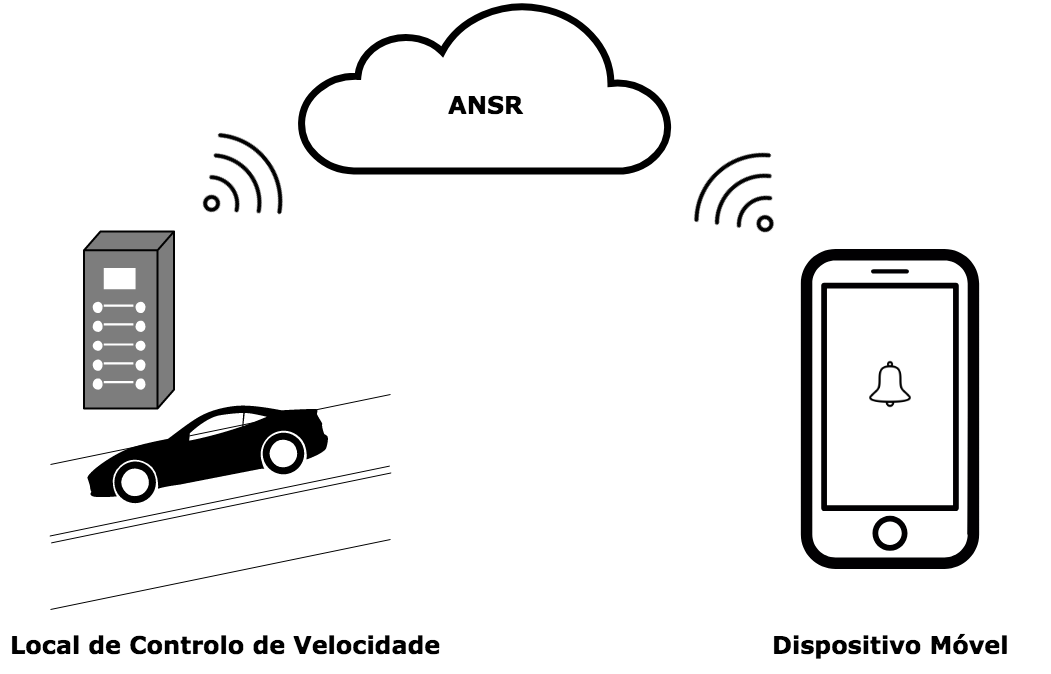
\includegraphics[scale=0.3]{./adoc_images/general_picture.png}
\caption{Imagem Geral}
\end{figure}

Atualmente o sistema de notificação de contraordenações por excesso de
velocidade é feito manualmente através de correio. Com este projeto
deverá ser possível ao cidadão subscrever os seus veículos através do
seu dispositivo móvel, possibilitando ser notificado de quaisquer
eventos que ocorram nos veículos registados. Este projeto é motivado
sobre a informação do evento de controlo de passagem de excesso de
velocidade, na expetativa que haja a redução de situações de violação do
excesso de velocidade. Através de uma plataforma móvel acreditamos ser
possível que o condutor fique mais atento à sua condução, dado que os
alertas recebidos são visualizados num espaço de tempo reduzido.

\hypertarget{_an_lise_do_problema_e_modelos}{%
\section{Análise do Problema e
Modelos}\label{_an_lise_do_problema_e_modelos}}

Dado a complexidade e diferentes aspetos presentes no objetivo deste
projeto, foi necessário fazer uma análise geral, uma investigação das
ferramentas a serem utilizadas e o estudo dos possíveis problemas.

\hypertarget{_an_lise}{%
\subsection{Análise}\label{_an_lise}}

O projeto irá consistir num Sistema Informático responsável por emitir
notificações de eventos para os dispositivos móveis, bem como processar
pedidos sobre informações relativas ao utilizador do dispositivo.\\
O Sistema Informático terá a responsabilidade de trabalhar dados
provenientes do sistema informático SINCRO . Só assim é possível ter
acesso aos eventos gerados pelos cinemómetro e já corretamente avaliados
e autorizados a serem notificados.\\
Também será necessária a realização da Componente Móvel (telemóvel, ou
outro dispositivo equivalente) através do qual o utilizador realizará
subscrição de eventos de contraordenação, de forma a receber as devidas
notificações dos mesmos.

\hypertarget{_ferramentas}{%
\subsection{Ferramentas}\label{_ferramentas}}

A \protect\hyperlink{big_picture}{figure\_title} apresenta uma vista
geral sobre o projeto.\\
O Sistema Informático irá ser criado numa linguagem que dê suporte para
aplicações servidoras (Java, Node.js, .NET, etc.). Relativamente aos
dispositivos móveis iremos usar uma linguagem que dê suporte a
multiplataforma (React Native, Xamarin, Native Script).

\hypertarget{_problemas}{%
\subsection{Problemas}\label{_problemas}}

A bateria limitada nos dispositivos móveis é algo a ter em conta na
realização deste projeto. Uma aplicação que utilize em grandes
quantidades a energia de um dispositivo pode ser facilmente posta em
causa e possivelmente desinstalada.\\
A quantidade e variedade de dispositivos móveis existentes no mercado é
também um dos problemas a considerar no projeto. Deverá ser desenvolvida
uma aplicação móvel (App) passível de ser utilizada por qualquer
condutor proprietário de um automóvel.

\begin{table}[]
	\centering
	\caption{My caption}
	\label{my-label}
	\begin{tabular}{@{}|l|l|@{}}
		\toprule
		\textbf{Problemas}                                                         & \textbf{Possiveis soluções}                                                                                                            \\ \midrule
		Poupança Bateria                                                           & \begin{tabular}[c]{@{}l@{}}Utilização de\\ notificações ‘Push’\end{tabular}                                                            \\ \midrule
		\begin{tabular}[c]{@{}l@{}}Variedade de\\ Dispositivos Móveis\end{tabular} & \begin{tabular}[c]{@{}l@{}}Utilizar uma linguagem\\ que possibilite a redução de código nativo, linguagem multiplataforma\end{tabular} \\ \bottomrule
	\end{tabular}
\end{table}

\hypertarget{_requisitos_funcionais}{%
\section{Requisitos Funcionais}\label{_requisitos_funcionais}}

No sistema SINCRO Mobile \footnote{Sistema de Gestão de Eventos de
  Contraordenação Por Excesso de Velocidade} serão implementados os
seguintes requisitos funcionais, presentes no
\protect\hyperlink{use_case}{figure\_title}. Cada requisito funcional
foi identificado com o indentificador RF \footnote{Requisito Funcional}
seguido pelo respetivo número.

\begin{figure}
\centering
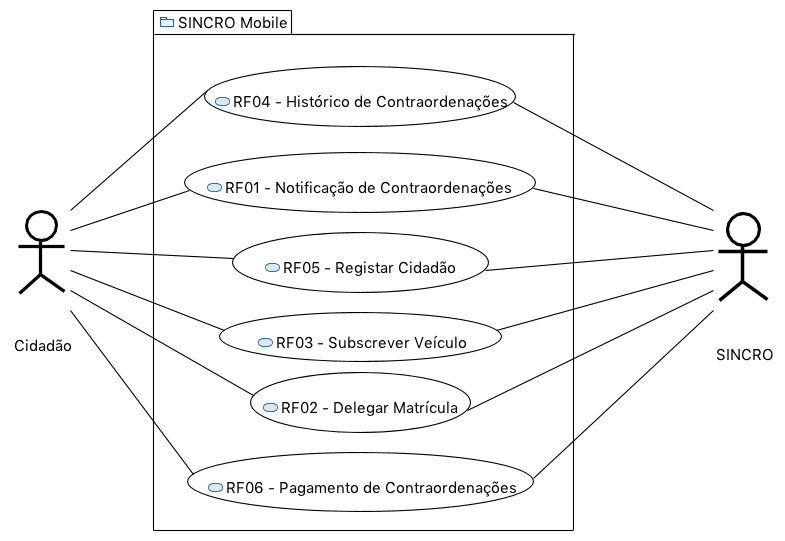
\includegraphics[scale=0.5]{./adoc_images/use_case.png}
\caption{Diagrama Caso de Uso}
\end{figure}

Para efetuar os mesmos será necessário a comunicação com a entidade
SINCRO . Quanto ao cidadão, este terá acesso a todas as funcionalidades.

\hypertarget{_rf01_notifica_o_de_contraordena_es}{%
\subsection{RF01 - Notificação de
Contraordenações}\label{_rf01_notifica_o_de_contraordena_es}}

O proprietário do veículo recebe a notificação acerca do evento no seu
telemóvel. As informações sobre o evento são enviadas pelo sistema
SINCRO .

\begin{figure}
\centering
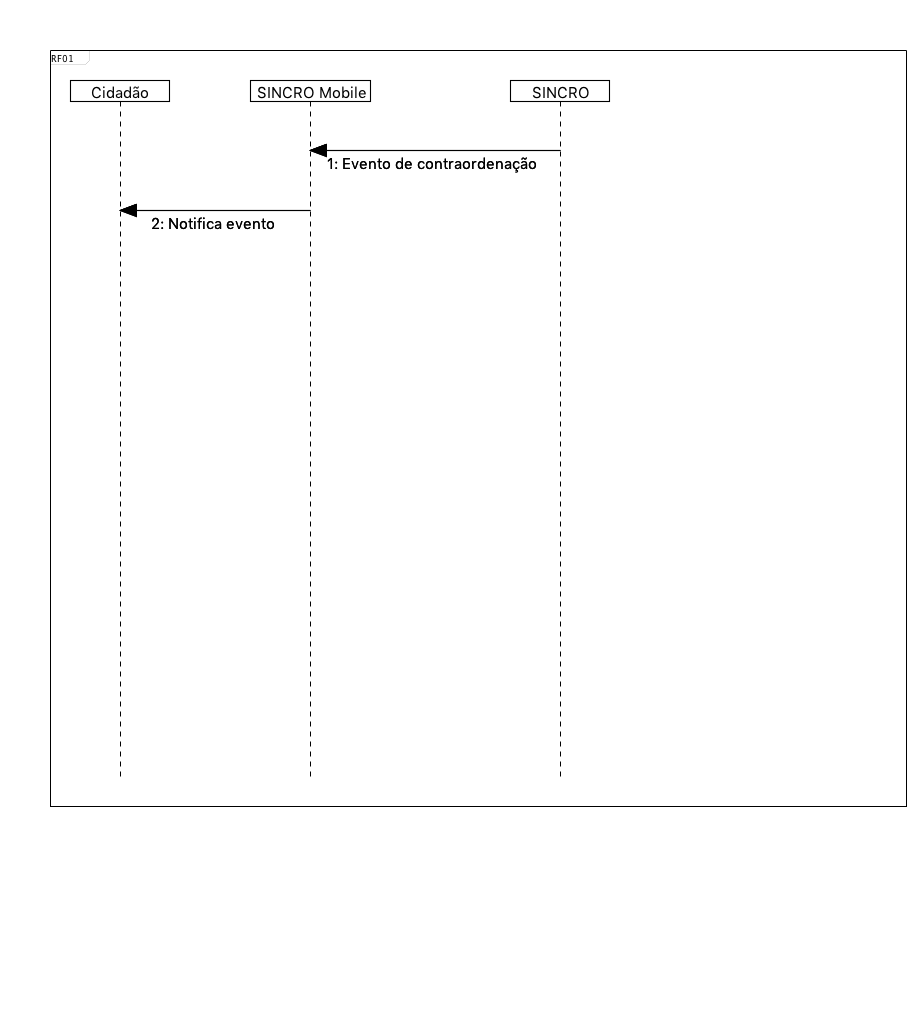
\includegraphics[scale=0.3]{./adoc_images/sequence/rf01.png}
\caption{Requisito Funcional I}
\end{figure}

\begin{enumerate}
\def\labelenumi{\arabic{enumi}.}
\item
  O evento de contraordenação é enviado do sistema SINCRO para o SINCRO
  Mobile onde irá ser guardado.\\
\item
  Posteriormente irá ser enviada uma notificação ao Cidadão com as
  informações sobre o respetivo evento.
\end{enumerate}

\hypertarget{_rf02_delegar_matr_cula}{%
\subsection{RF02 - Delegar Matrícula}\label{_rf02_delegar_matr_cula}}

Permite o utilizador delegar o seu veículo a outro utilizador, já
registado no sistema, que aceite esta responsabilidade.

\begin{figure}
\centering
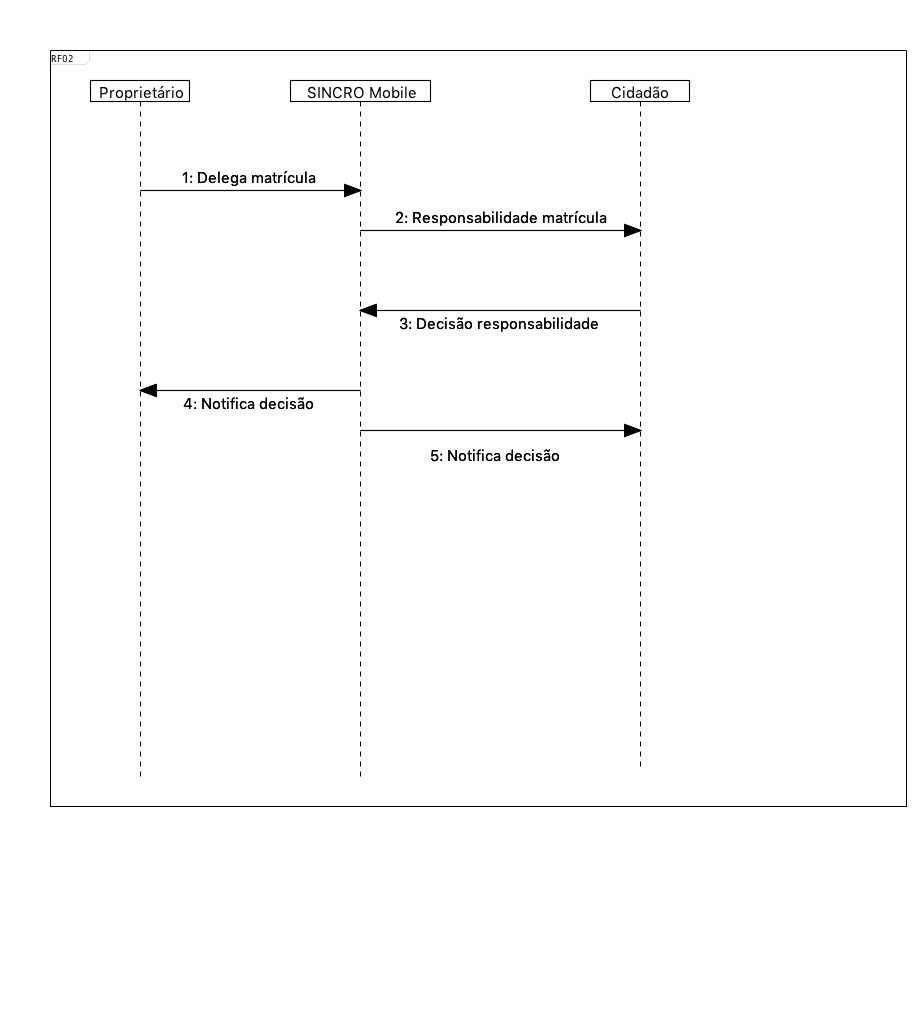
\includegraphics[scale=0.3]{./adoc_images/sequence/rf02.png}
\caption{Requisito Funcional II}
\end{figure}

\begin{enumerate}
\def\labelenumi{\arabic{enumi}.}
\item
  Envio do pedido de delegação por parte do Proprietário. Onde irá
  constar a respetiva matrícula e o Cidadão a quem delega a
  responsabilidade.
\item
  O Cidadão irá receber um pedido para aceitar a responsabilidade do
  veículo.
\item
  O Cidadão envia decisão face a responsabilidade.
\item
  Se o Cidadão aceitar a responsabilidade (3), deverá ser entregue ao
  proprietário uma notificação de sucesso. Caso contrário irá receber
  uma notificação de insucesso.
\item
  Se o Cidadão aceitar a responsabilidade (3), o mesmo irá receber uma
  notificação sobre o veículo e respetiva matrícula pelo qual é
  responsável. Caso contrário a notificação não terá efeito.
\end{enumerate}

\hypertarget{_rf03_subscrever_ve_culo}{%
\subsection{RF03 - Subscrever Veículo}\label{_rf03_subscrever_ve_culo}}

Depois de registado, o utilizador poderá subscrever as suas viaturas,
bem como viaturas delegadas por outros utilizadores. Passando a ser o
responsável por quaisquer futuros eventos.

\begin{figure}
\centering
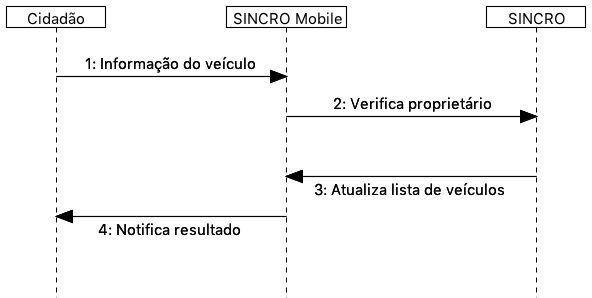
\includegraphics[scale=0.3]{./adoc_images/sequence/rf03.png}
\caption{Requisito Funcional III}
\end{figure}

\begin{enumerate}
\def\labelenumi{\arabic{enumi}.}
\item
  Envio da matrícula e dados que possam identificar o veículo a
  subscrever.
\item
  Informação é enviada para o sistema SINCRO onde irá ser verificada a
  autenticidade do proprietário.
\item
  Lista de veículos do Cidadão é atualizada com base no resultado do
  passo anterior (2).
\item
  Cidadão é notificado com o resultado da operação.
\end{enumerate}

\hypertarget{_rf04_hist_rico_de_contraordena_es}{%
\subsection{RF04 - Histórico de
Contraordenações}\label{_rf04_hist_rico_de_contraordena_es}}

É disponibilizada uma lista de contraordenações com os últimos eventos
ocorridos. O utilizador poderá visualizar os eventos de contraordenação
e aceder à sua informação.

\begin{figure}
\centering
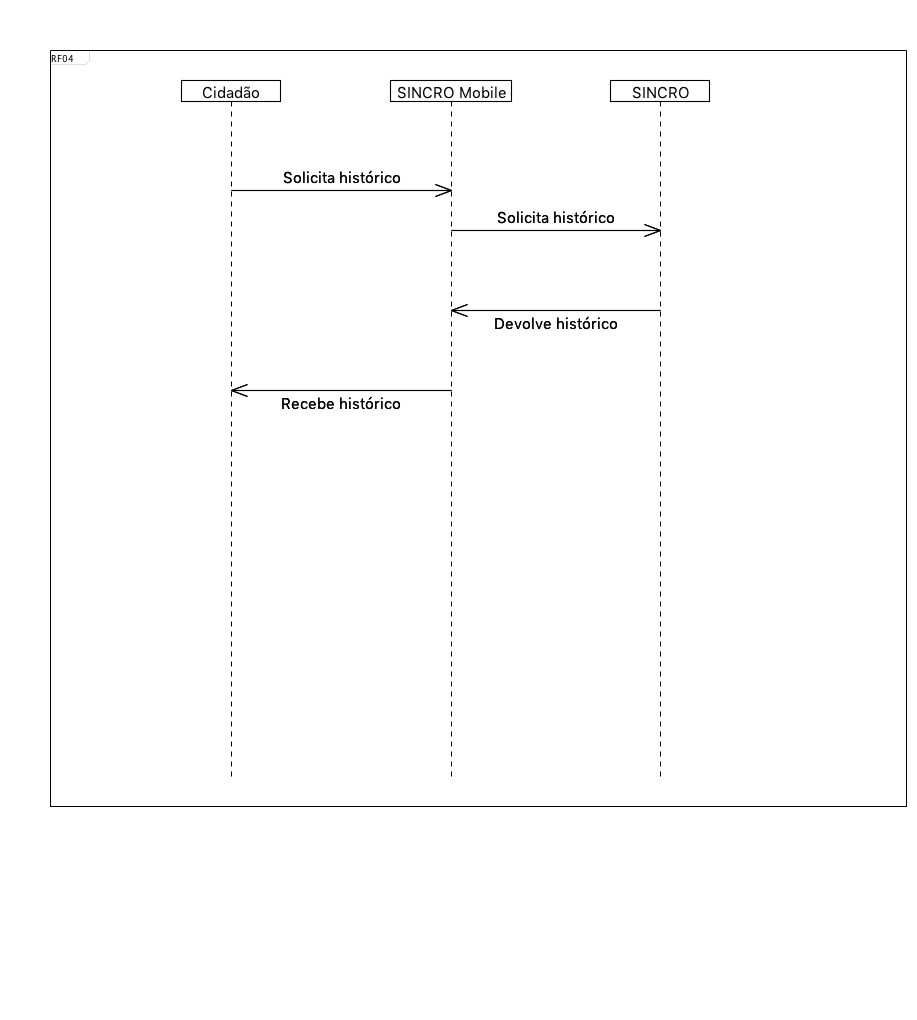
\includegraphics[scale=0.3]{./adoc_images/sequence/rf04.png}
\caption{Requisito Funcional IV}
\end{figure}

\begin{enumerate}
\def\labelenumi{\arabic{enumi}.}
\item
  Pedido de histórico do Cidadão.
\item
  Envio do pedido (1) para o sistema SINCRO .
\item
  É devolvido ao SINCRO Mobile o histórico do Cidadão.
\item
  Cidadão recebe histórico de contraordenações.
\end{enumerate}

\hypertarget{_rf05_registar_cidad_o}{%
\subsection{RF05 - Registar Cidadão}\label{_rf05_registar_cidad_o}}

Para ter acesso a quaisquer funcionalidades é necessário o cidadão se
registar no sistema através do seu cartão de cidadão e do seu contacto
telefónico de forma a ser identificável pelo sistema.

\begin{figure}
\centering
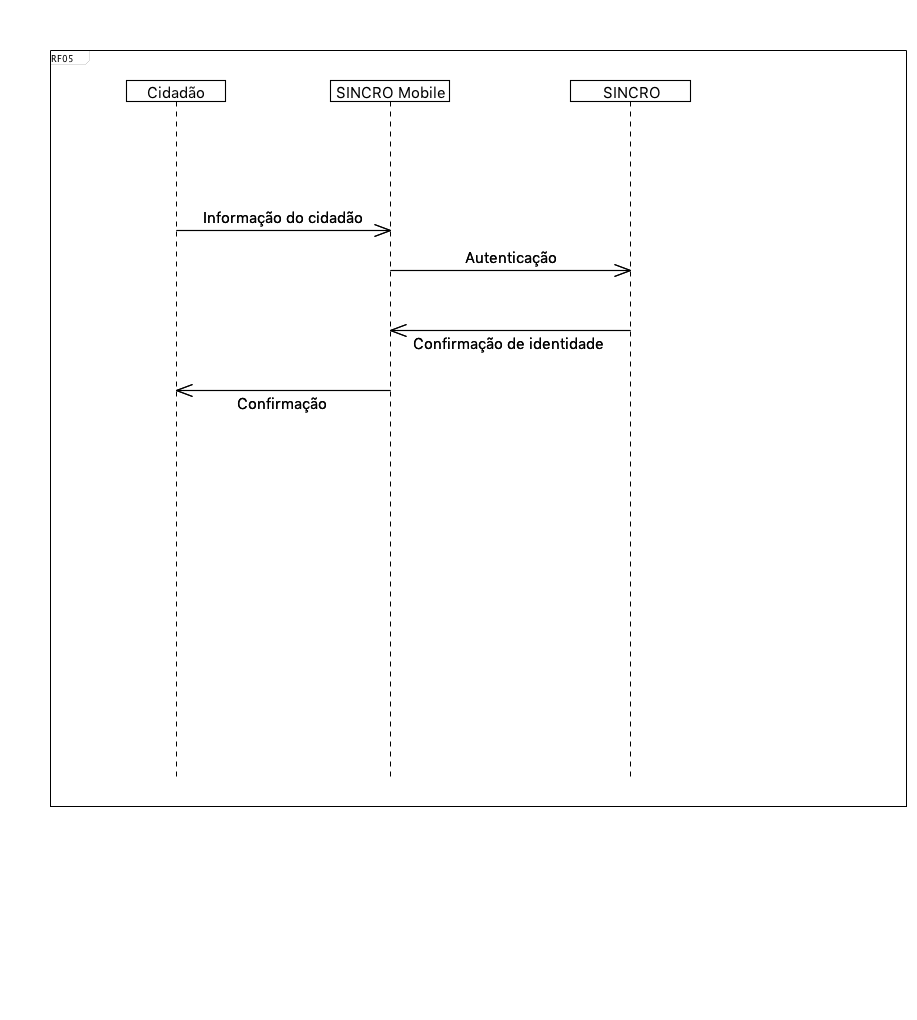
\includegraphics[scale=0.3]{./adoc_images/sequence/rf05.png}
\caption{Requisito Funcional V}
\end{figure}

\begin{enumerate}
\def\labelenumi{\arabic{enumi}.}
\item
  Envio dos dados do Cidadão (nome, cartão de cidadão, morada, número,
  etc).
\item
  Verificação da validade da identidade do Cidadão.
\item
  Se a identidade for verificada com sucesso pelo sistema SINCRO é
  adicionado um novo utilizador. Em caso de insucesso não ocorre
  alteração nenhuma.
\item
  Cidadão recebe confirmação do seu registo. Caso o passo (3) tenha
  resultado em insucesso, o seu registo é rejeitado.
\end{enumerate}

\hypertarget{_rf06_pagamento_de_contraordena_es}{%
\subsection{RF06 - Pagamento de
Contraordenações}\label{_rf06_pagamento_de_contraordena_es}}

Será disponibilizado para qualquer contraordenação a possibilidade de
pagamento do valor respetivo da mesma.

\begin{figure}
\centering
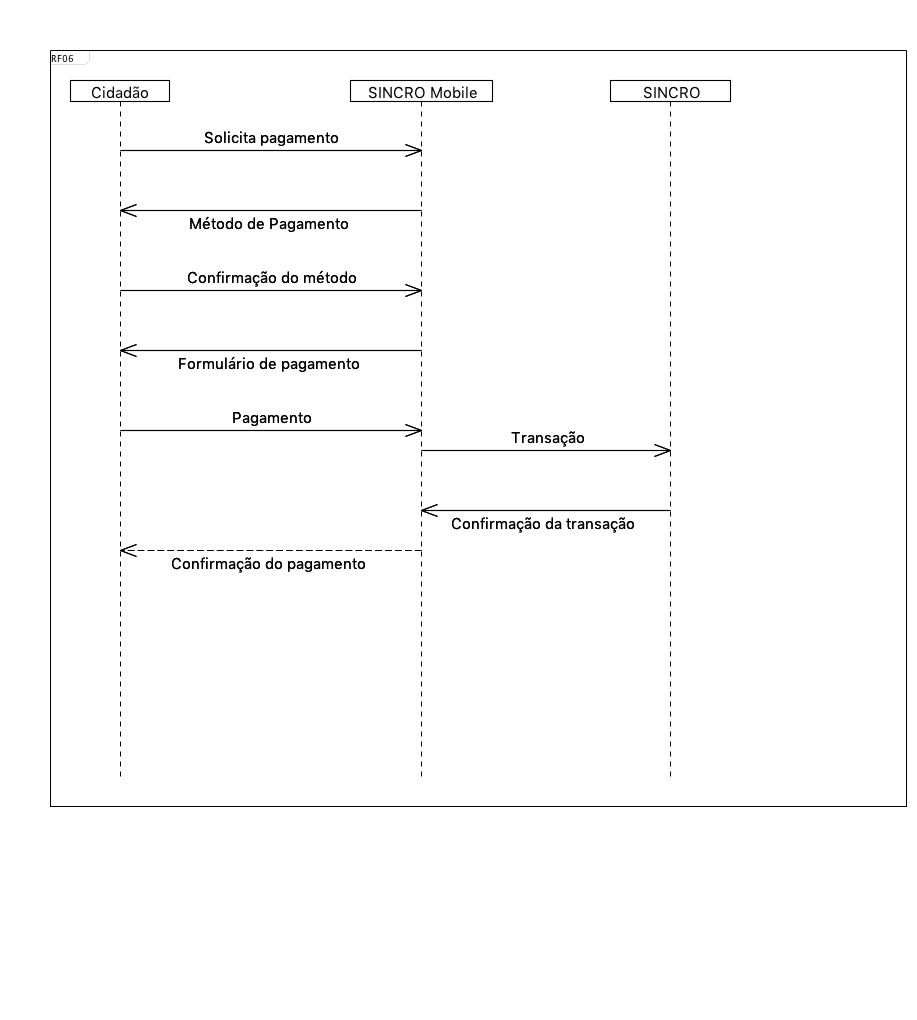
\includegraphics[scale=0.3]{./adoc_images/sequence/rf06.png}
\caption{Requisito Funcional VI}
\end{figure}

\begin{enumerate}
\def\labelenumi{\arabic{enumi}.}
\item
  Envio do pedido de pagamento.
\item
  São disponibilizadas as formas de pagamento que o Cidadão poderá
  escolher.
\item
  É confirmado o método de pagamento
\item
  Envio do formulário de pagamento. No qual o utilizador poderá
  verificar os valores de pagamento e a respetiva contraordenação que
  pretende saldar.
\item
  Confirmação de pagamento é enviada.
\item
  Transação monetária é feita através do sistema SINCRO .
\item
  Confirmação é enviada em caso de sucesso da transação (6).
\item
  Cidadão é notificado com o resultado do pagamento da contraordenação.
\end{enumerate}

\hypertarget{_requisitos_n_o_funcionais}{%
\section{Requisitos Não Funcionais}\label{_requisitos_n_o_funcionais}}

Todas as garantias necessárias de realizar de forma possibilitar a
implementação dos requisitos não funcionais são do nosso interesse.
Contudo não nos comprometemos com a realização das mesmas.

\hypertarget{_rnf01_escalabilidade}{%
\subsection{RNF01 - Escalabilidade}\label{_rnf01_escalabilidade}}

O sistema irá ser desenhado de forma a suportar múltiplos acessos por
vários utilizadores. Deverão ser utilizadas técnicas como o
balanceamento de carga e distribuição de operações de forma a resultar
num melhor desempenho dp sistema.

\hypertarget{_rnf02_seguran_a}{%
\subsection{RNF02 - Segurança}\label{_rnf02_seguran_a}}

Dada a importância deste tipo de informação apresentado na aplicação,
deverão ser usadas formas de possibilitar a máxima segurança no sistema.

\hypertarget{_rnf03_toler_ncia_a_falhas}{%
\subsection{RNF03 - Tolerância a
falhas}\label{_rnf03_toler_ncia_a_falhas}}

O cidadão irá usar o nosso sistema para efetuar pagamentos e aceder a
informação importante. Deverá ser garantido o bom funcionamento da nossa
aplicação e irá ser dado suporte para possíveis falhas.

\hypertarget{_rnf04_rapidez_de_entrega}{%
\subsection{RNF04 - Rapidez de
Entrega}\label{_rnf04_rapidez_de_entrega}}

Uma vez que o sistema funcionará todo através de sistemas informáticos,
vai ser possível uma entrega ao utilizador mais rápida, dos eventos de
contraordenação.

\hypertarget{_arquitetura_do_projeto}{%
\section{Arquitetura do Projeto}\label{_arquitetura_do_projeto}}

Com base no objetivo do sistema SINCRO Mobile foi necessário desenhar
uma arquitetura precisa do projeto.

\begin{figure}
\centering
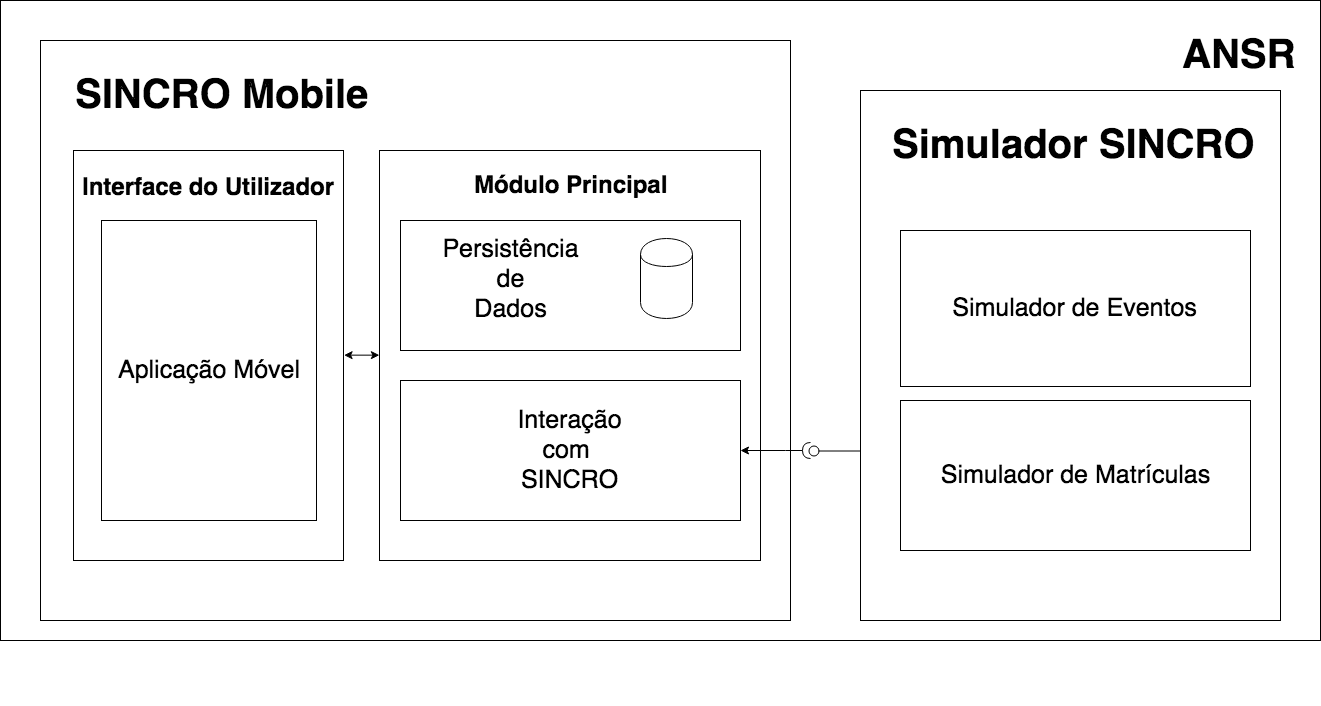
\includegraphics[scale=0.3]{./adoc_images/block_diagram.png}
\caption{Arquitetura do Projeto}
\end{figure}

Na \protect\hyperlink{arquiteture}{figure\_title} é possível visualizar
os componentes presentes na arquitetura e as interligações das mesmas.

\hypertarget{_m_dulo_principal}{%
\subsection{Módulo Principal}\label{_m_dulo_principal}}

O Módulo Principal irá ser responsável por implementar todas as
funcionalidades disponíveis no SINCRO Mobile . Todos os componentes
envolvidos no sistema irão desempenhar funções com base nas decisões do
Módulo Principal.

\hypertarget{_persist_ncia_de_dados}{%
\subsection{Persistência de Dados}\label{_persist_ncia_de_dados}}

A componente de Persistência de Dados tem a responsabilidade de garantir
a segurança dos dados, bem como o controlo do acesso aos mesmos.\\
Como está presente na imagem, o Módulo principal irá efetuar o acesso a
dados e a alteração dos mesmos. Quanto ao componente de Interação com o
sistema SINCRO , este irá apenas realizar alteração dos dados.

\hypertarget{_interface_do_utilizador}{%
\subsection{Interface do Utilizador}\label{_interface_do_utilizador}}

Esta componente é constituída por duas componentes internas. Uma
componente aplicacional realizada para dispositivos móveis e outra
componente para web.\\
A Aplicação Móvel irá funcionar como interface para o cidadão utilizador
das funcionalidades presentes no sistema SINCRO Mobile .\\
A componente Aplicação Web vai ser de realização opcional. Será
construída com o propósito de disponibilizar informação interna passível
de ser utilizada para consulta de \emph{mensagens de log}.

\hypertarget{_intera_o_com_sincro}{%
\subsection{Interação com SINCRO}\label{_intera_o_com_sincro}}

Tem como função principal interagir com o sistema SINCRO para a
realização de funcionalidades presentes no nosso sistema que exijam
funcionalidades presentes na interface SINCRO.

\hypertarget{_interface_de_comunica_o_com_sincro}{%
\subsection{Interface de Comunicação com
SINCRO}\label{_interface_de_comunica_o_com_sincro}}

O sistema SINCRO contém informações das quais não poderemos ter acesso.
Será necessário criar esta interface para que seja possível simular a
comunição com o mesmo.\\
A mesma irá ser bastante útil na realização de testes e bom
funcionamento do sistema SINCRO Mobile .

\hypertarget{_implementa_o_do_sistema_sincro_mobile}{%
\section{Implementação do Sistema SINCRO
Mobile}\label{_implementa_o_do_sistema_sincro_mobile}}

Nesta secção são descritas as técnologias utilizadas no desenvolvimento
do SINCRO Mobile bem como a razão da sua adoção, discriminando as ditas
técnologias por camada aplicacional: dados, negócio e cliente.\\
A camada de negócio é referente ao Sistema Central, a camada de dados à
Persistencia de dados, e o cliente à Interface Humana.

\hypertarget{_m_dulo_principal_2}{%
\subsection{Módulo Principal}\label{_m_dulo_principal_2}}

\begin{itemize}
\item
  \protect\hyperlink{Java}{{[}Java{]}}\\
  É uma técnologia amplamente utilizada. O seu código é compilado para
  \emph{bytecode} e executado numa máquina virtual, a JVM o que fornece
  uma camada de abstação independente da plataforma onde corre.
\end{itemize}

\hypertarget{_camada_de_dados}{%
\subsection{Camada de dados}\label{_camada_de_dados}}

A camada de dados baseia-se num sistema de gestão de base de dados
(SGBD). Neste projeto, o sistema de gestão de base de dados a ser usado
deverá ser o \emph{PostgreSQL Server}, sendo um dos motivos para a sua
escolha o facto de estar disponível na comunidade OpenSource.\\

\begin{itemize}
\item
  \protect\hyperlink{FrameworkHybernate}{{[}FrameworkHybernate{]}}\\
  O \emph{Hybernate} é uma biblioteca desenvolvida para Java com o
  intuito de forncer uma \emph{framework} que permitisse mapear objetos
  pertencentes ao \emph{modelo de dominio} em objetos equivalentes no
  respetivo \emph{modelo relacional}.
\end{itemize}

\hypertarget{_camada_de_neg_cio}{%
\subsection{Camada de negócio}\label{_camada_de_neg_cio}}

A camada de negócio representa o \emph{core} do sistema. Nesta camada é
usada a \emph{framework Spring}.

\begin{itemize}
\item
  \protect\hyperlink{Spring}{{[}Spring{]}}\\
  O \emph{Spring} é uma \emph{framework} desenvolvida para java, sendo
  constituida por diversos módulos que oferecem uma gama de serviços
  abrangente.
\end{itemize}

\hypertarget{_camada_cliente}{%
\subsection{Camada Cliente}\label{_camada_cliente}}

A camada cliente representa a componente aplicacional, que neste caso é
uma aplicação móvel.

\begin{itemize}
\item
  \protect\hyperlink{ReactNative}{{[}ReactNative{]}}\\
  O \emph{React Navtie} é uma tecnologia de desenvolvimento de
  aplicações móveis nativas para multiplataforma (Android e iOS) em que
  práticamente todo o o código é partilhado entre as duas versões. É
  usado \emph{javascript} para o desenvolvimento de aplicações nesta
  técnlogia bem como um \emph{framework} baseado em \emph{React} .
\end{itemize}

\hypertarget{_conclus_o}{%
\section{Conclusão}\label{_conclus_o}}

Neste documento é descrito um sistema cujo objetivo é futuramente ser de
alguma forma integrado na rede ANSR, pelo que é necessário que a sua
implementação seja de certo modo visada na sua futura manutenção. Por
essa razão é necessário um cuidado acrescido na legibilidade do código
desenvolvido, bem como a facilidade da sua alteração.

\hypertarget{_anexos}{%
\section{Anexos}\label{_anexos}}

\hypertarget{_cronograma}{%
\subsection{Cronograma}\label{_cronograma}}

O desenvolvimento do projeto está a decorrer da forma prevista, estando
portanto a cumprir o cronograma proposto. Na
\protect\hyperlink{cronograma}{figure\_title} é apresentado o progresso
em relação às tarefas propostas que já foram realizadas ou estão ainda
por realizar.

\begin{figure}
\centering
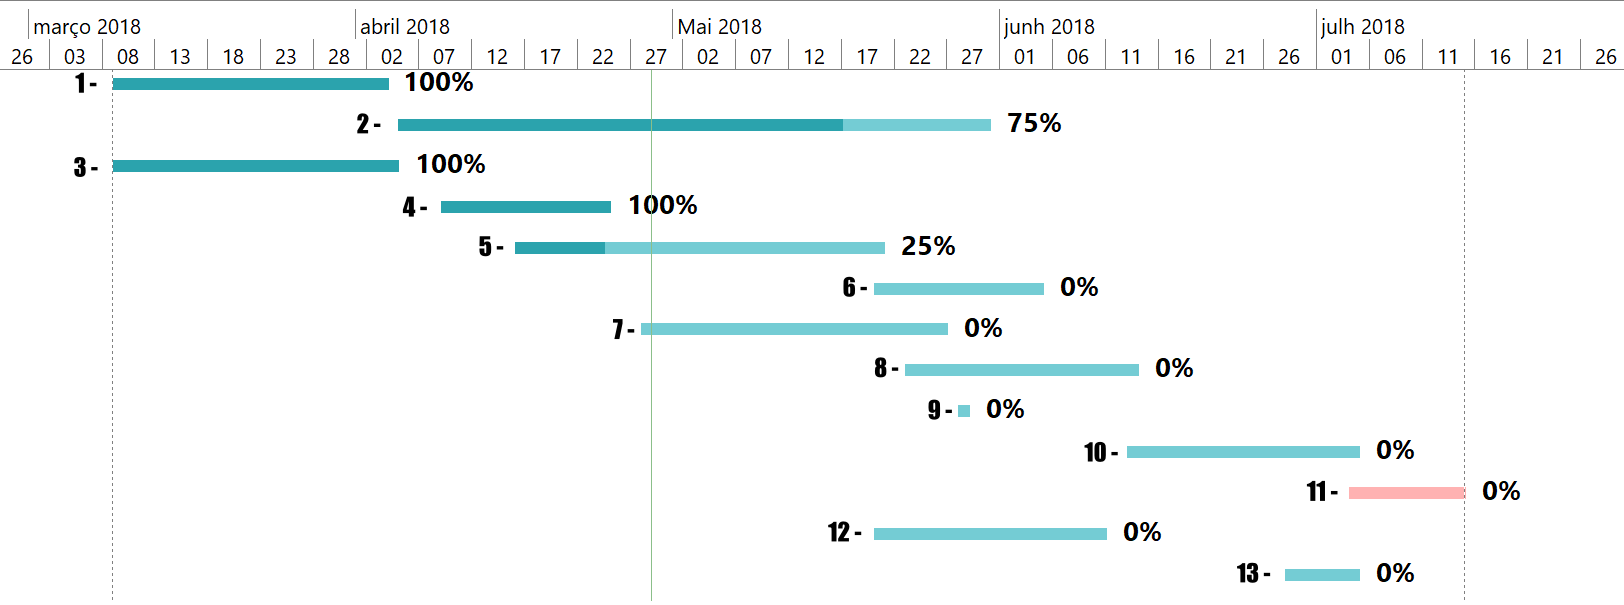
\includegraphics[scale=0.22]{./adoc_images/cronograma_dates.png}
\caption{Cronograma do Projeto}
\end{figure}

\hypertarget{_tarefas}{%
\subsubsection{Tarefas}\label{_tarefas}}

\begin{enumerate}
\def\labelenumi{\arabic{enumi}.}
\item
  Levantamento e análise de requisitos funcionais e não funcionais.

  \begin{itemize}
  \item
    Tarefa realizada a 100\%.
  \end{itemize}
\item
  Desenho da arquitetura do sistema a desenvolver.

  \begin{itemize}
  \item
    Tarefa realizada a 100\%, mas poderão ocurrer alterações ao longo do
    decorrer do projeto.
  \end{itemize}
\item
  Especificação do sistema a desenvolver.

  \begin{itemize}
  \item
    Tarefa realizada a 100\%.
  \end{itemize}
\item
  Avaliação do quadro tecnológico a utilizar.

  \begin{itemize}
  \item
    Tarefa realizada a 100\%.
  \end{itemize}
\item
  Desenvolvimento dos elementos do sistema.

  \begin{itemize}
  \item
    Tarefa iniciada.
  \end{itemize}
\item
  Testes do sistema desenvolvido.
\item
  Desenvolvimento da aplicação móvel.
\item
  Testes funcionais da aplicação móvel.
\item
  Entrega da versão beta.
\item
  Resolução de \emph{bugs} e melhoria de código.
\item
  Melhoria de aspetos não funcionais da aplicação.
\item
  Resolução de aspetos específicos dos sistemas operativos móveis.
\item
  Interface de pagamento (Opcional).
\end{enumerate}

\hypertarget{_refer_ncias}{%
\section{Referências}\label{_refer_ncias}}

\begin{itemize}
\item
  {[}Java{]} \url{https://www.java.com}
\item
  {[}FrameworkHybernate{]} \url{http://hibernate.org}
\item
  {[}Spring{]} \url{https://spring.io/}
\item
  {[}ReactNative{]} \url{https://facebook.github.io/react-native/}
\end{itemize}

\end{document}
